

\section{Daten}
\label{sec:daten}

F\"ur die Erprobung verschiedener Machine Learning Modelle wurde vom LQM der Datensatz
\textit{da\_242} f\"ur die Studienrichtungen \textit{Bachelorstudium P\"adagogik},
\textit{Bachelorstudium Betriebswirtschaft} und \textit{Diplomstudium Rechtswissenschaften} bereitgestellt.
Die betrachteten Jahre sind die Studienjahre 2015/2016 bis 2019/2020, somit also f\"unf Jahre.

Der Datensatz beinhaltet Daten von ca. 40 000 Studienjahren. Das bedeutet, dass jede studierende Person,
welche \"uber mehrere Jahre in einer der beobachteten Studienrichtungen inskribiert war, auch mehrere Eintr\"age im Datensatz besitzt.

Insgesamt gibt es pro Studentin oder Student und Studienjahr ca. 100 Merkmale.
F\"ur die tats\"achliche Vorhersage durch die Machine Learning Modelle wurden nur wenige davon verwendet.
Der Grund daf\"ur war, dass die verworfenen Merkmale gro{\ss}teils unvollst\"andig f\"ur den gesamten Datensatz waren
und dass sie oft keine weiteren Informationen zu den verwendeten Merkmalen beinhaltet haben. Jene Merkmale, mit welchen hautps\"achlich
gearbeitet wurde, sind in der \hyperref[tab:name]{Tabelle 1.1} zusammengefasst und mit ihren Labels beschrieben. Die Eigenschaften, welche mit
*  gekennzeichnet sind, versucht man vorherzusagen.

\begin{table}[ht]
  \caption{\label{tab:name} Eigenschaften der Studierenden und deren Auspr\"agung}
  \begin{tabular}{ p{1cm} p{7cm}  p{5cm} }
    \toprule
    $E_i$     & Name                                & Ausprägungen     \\
    \midrule
    $E_1$     & Aktuelles Studienjahr               & numerisch        \\
    $E_2$     & Matrikelnummer                      & numerisch        \\
    $E_3$     & Geschlecht                          & binär            \\
    $E_4$     & Besuchter Schultyp                  & one-hot-encoding \\
    $E_5$     & Verspätet angemeldet                & binär            \\
    $E_6$     & Herkunft                            & one-hot-encoding \\
    $E_7$     & Inskription in mehreren Studien     & numerisch        \\
    $E_8$     & Jahre seit Matura                   & numerisch        \\
    $E_9$     & Jahre seit 18                       & numerisch        \\
    $E_{10}$  & ECTS pro Semester                   & numerisch        \\
    $E_{11}$  & Vorbildung der Eltern               & binär            \\
    $E_{12}$  & ECTS im Jahr zuvor (wenn vorhanden) & numerisch        \\
    $E_{13}$  & Studienart                          & one-hot-encoding \\
    $E_{14}$  & Erste Prüfung negativ               & binär            \\
    $E_{15}$  & Geplante Mindeststudienzeit         & numerisch        \\
    $E_{16}$  & Bisherige Studiendauer in Semestern & numerisch        \\
    $E_{17}*$ & Studienstatus kommendes Jahr        & nominal          \\
    $E_{18}*$ & ECTS dieses Jahr                    & numerisch        \\
    $E_{19}*$ & Semesterwochenstunden dieses Jahr   & numerisch        \\
    $E_{20}*$ & Aktiv oder nicht                    & binär            \\
    \bottomrule
  \end{tabular}

\end{table}

Grunds\"atzlich sind die Merkmale \textit{\glqq weiterer Studienstatus\grqq{}},
\textit{\glqq ECTS in diesem Jahr\grqq{}}, \textit{\glqq Semesterwochenstunden in diesem Jahr\grqq{}} und
\textit{\glqq pr\"ufungsaktiv oder nicht\grqq{}} erst nach einem absolvierten Studienjahr verf\"ugbar. Somit sind diese Merkmale,
die bereits bekannten Zielwerte der Daten. Das Ziel der Vorhersagemodelle ist es, aus vorhandenen Trainingsdaten eine verl\"assliche
Regel zu lernen, um diese Werte f\"ur neue Daten ohne gegebene Zielwerte zu
sch\"atzen. Die anderen Merkmale k\"onnen, je nach N\"utzlichkeit zur Vorhersage, als Input
in den Modellen verwendet werden oder nicht.

Die Merkmale unterscheiden sich auch hinsichtlich ihrer Ver\"anderbarkeit im zeitlichen Verlauf. Eigenschaften wie \textit{\glqq Studienrichtung\grqq{}},
\textit{\glqq Geschlecht\grqq{}}, \textit{\glqq Herkunft\grqq{}} oder \textit{\glqq besuchter Schultyp\grqq{}} ver\"andern sich im Laufe der Zeit nicht und bleiben \"uber die Studienzeit gleich.
Im Gegensatz dazu \"andern sich \textit{\glqq kumulierte ECTS\grqq{}} oder \textit{\glqq ECTS im Jahr zuvor\grqq{}} in jedem Studienjahr.

Deswegen werden Ans\"atze ausprobiert, die nur auf unver\"anderbaren Merkmalen beruhen. Weiters werden Ans\"atze formuliert, wo versucht wird
die ver\"anderlichen Merkmale bestm\"oglich zu verwenden.

Die Pr\"ufungsaktivit\"at kann, wie oben beschrieben, mehrere Einflussfaktoren haben. Einer dieser Faktoren ist der Abschluss des Studiums. Das ist in zweierlei Hinsicht interessant.
Auf der einen Seite bedeutet ein Studienabschluss, dass man zwar in diesem Studienjahr pr\"ufungsaktiv sein wird, jedoch danach auch sein Studium beendet hat.
Dadurch kann man in weiterer Folge in den darauffolgenden Jahren nicht mehr pr\"ufungsaktiv sein.
Auf der anderen Seite ben\"otigt man f\"ur einen Studienabschluss eine festgelegte Anzahl an kumulierter, positiv absolvierter ECTS. Dadurch besteht die
M\"oglichkeit, nur durch den Abschluss des Studiums pr\"ufungsaktiv zu sein erst, wenn man gen\"ugend ECTS erreicht hat, und nicht schon ab dem ersten Studienjahr.
Da die Anzahl an ECTS, die man f\"ur einen Abschluss erreichen muss, nach Studienrichtung variert, ist in \hyperref[fig:abb1]{Abbildung 1.1}
der Anteil an pr\"ufungsaktiven Studierenden nach Studienjahr dargestellt.

\begin{figure}[ht]
  \label{fig:abb1}
  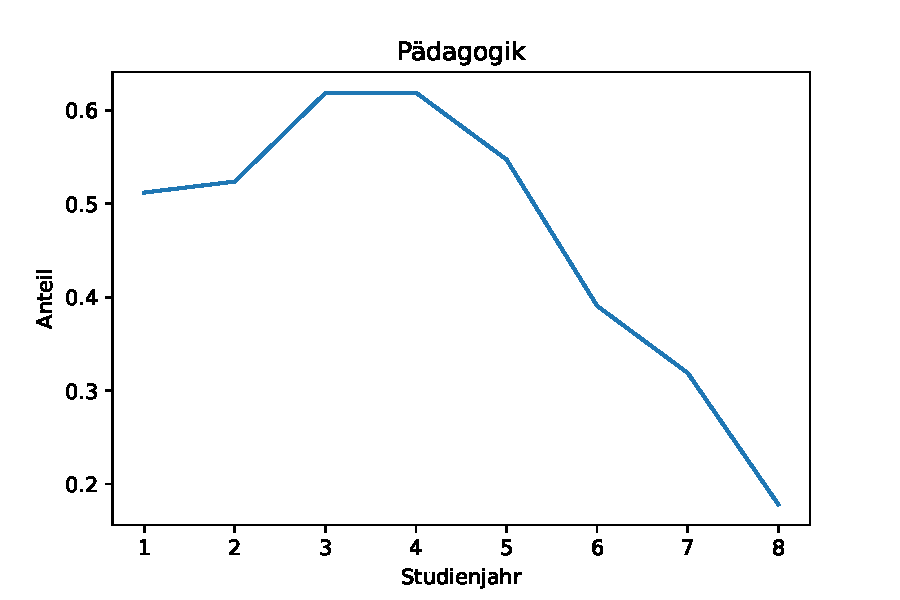
\includegraphics[width = 0.5\columnwidth]{pad1.pdf}
  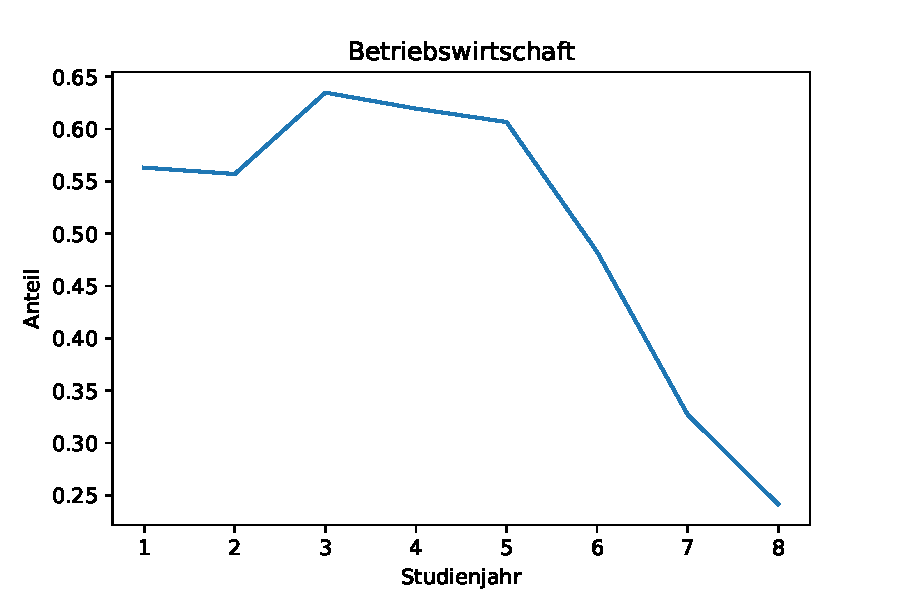
\includegraphics[width = 0.5\columnwidth]{bwl1.pdf}
  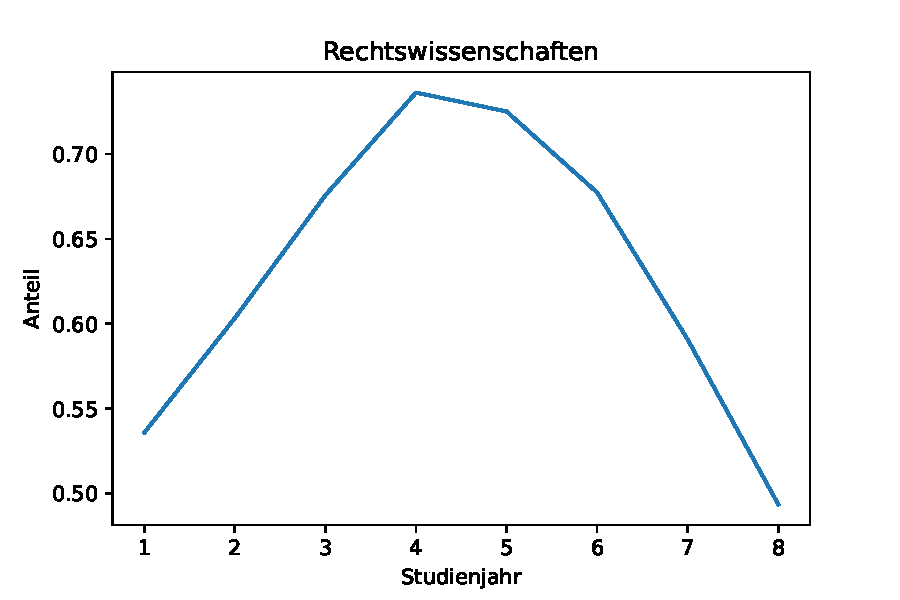
\includegraphics[width = 0.5\columnwidth]{jus1.pdf}
  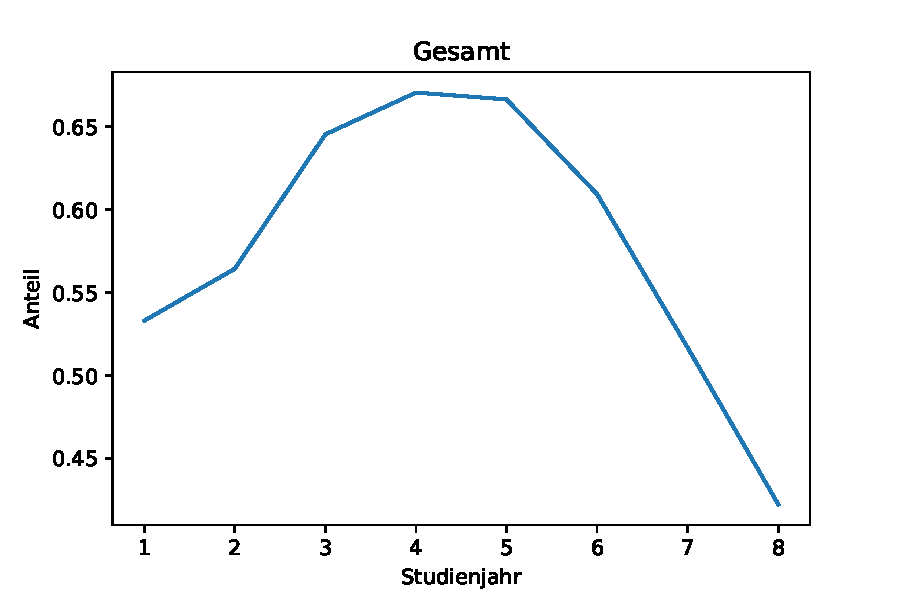
\includegraphics[width = 0.5\columnwidth]{ges1.pdf}
  \caption[Anteil an pr\"ufungsaktiven Studierenden nach Studienjahr und -richtung]{Der Anteil an pr\"ufungsaktiven Studierenden an insgesamt Studierenden, die noch bis ins jeweilige
    Studienjahr verblieben sind. In der Grafik \textit{Gesamt} wird ein gewichteter
    Anteil nach Studienrichtung gezeigt.}
\end{figure}

Eine Grundannahme in s\"amtlichen erprobten Ans\"atzen ist, dass Studierende, von denen man Anzahl und Merkmalskombinationen genau kennt, auch in einem Zeitrahmen von
drei Jahren in der Zukunft auch noch einen beachtlichen Anteil an den pr\"ufungsaktiven Studierenden bilden werden. Diese Annahme wird gest\"utzt, weil man, wie in \hyperref[fig:abb2]{Abbildung 1.2}
dargestellt, sieht, dass der Anteil an pr\"ufungsaktiven Studierenden aus h\"oheren Studienjahren tats\"achlich gro{\ss} ist. W\"are das nicht der Fall, m\"usste man sich nicht mit
P1 auseinandersetzen.

\begin{figure}[ht]
  \label{fig:abb2}
  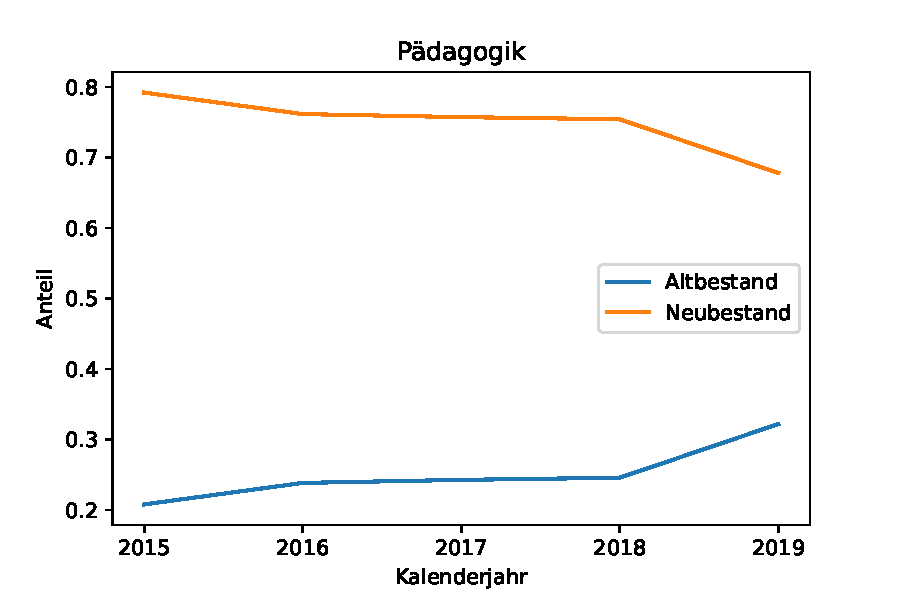
\includegraphics[width = 0.5\columnwidth]{pad2.pdf}
  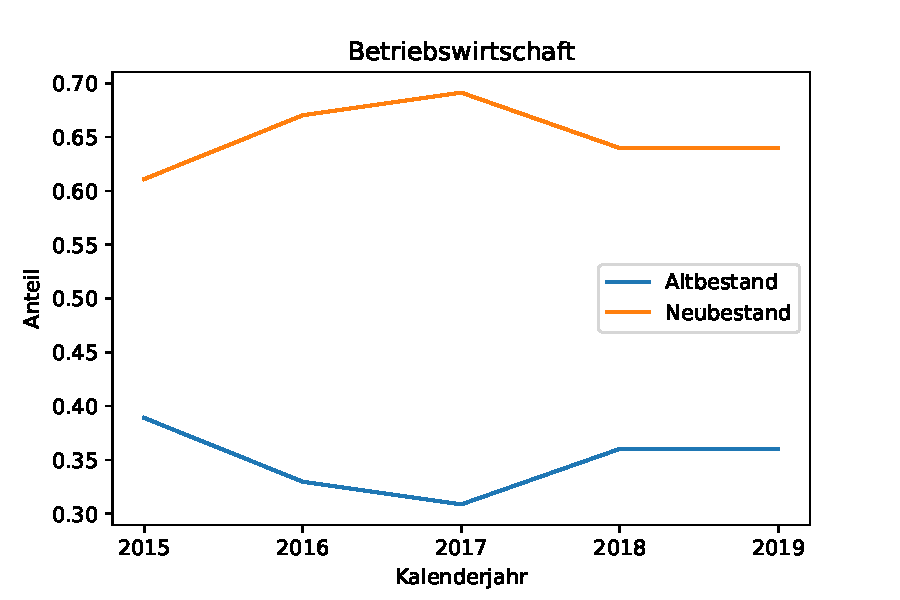
\includegraphics[width = 0.5\columnwidth]{bwl2.pdf}
  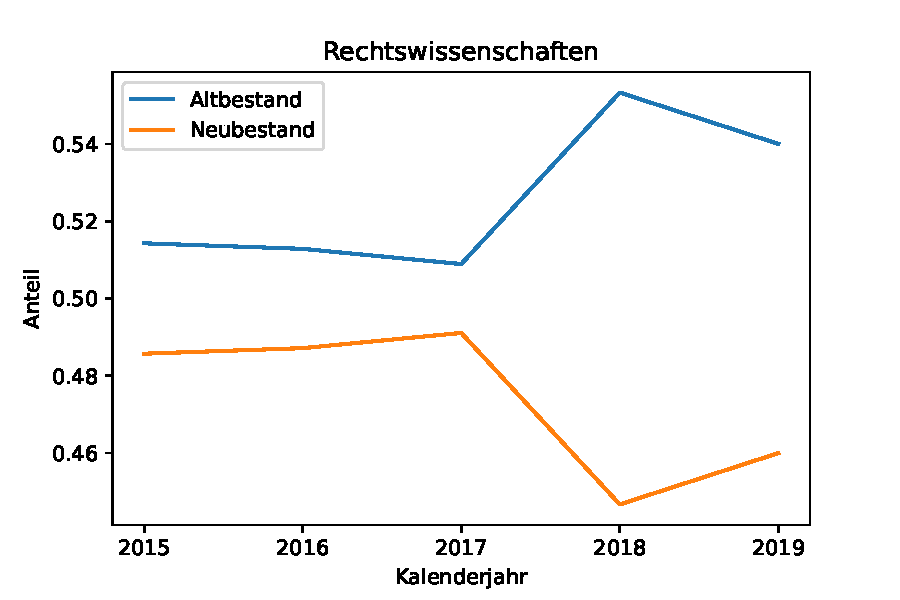
\includegraphics[width = 0.5\columnwidth]{jus2.pdf}
  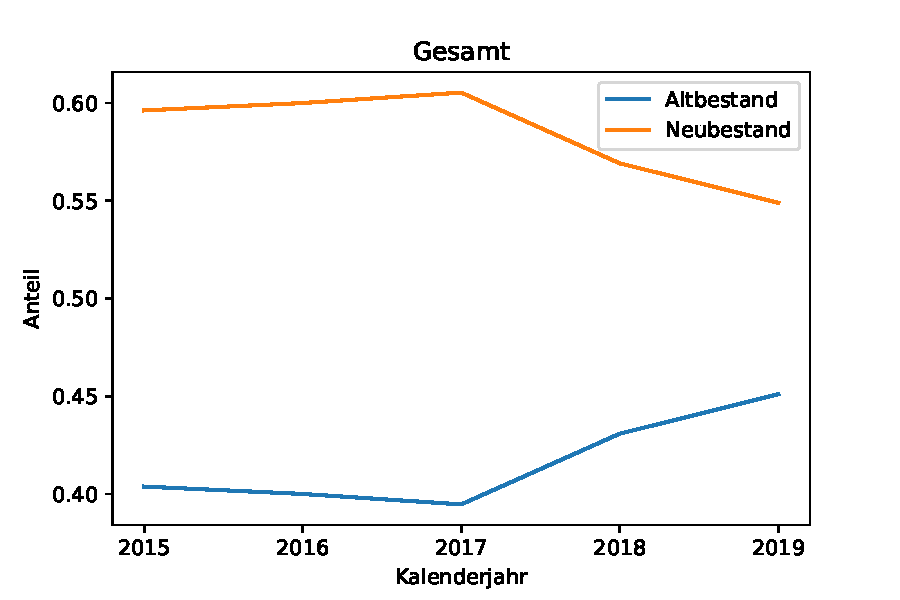
\includegraphics[width = 0.5\columnwidth]{ges2.pdf}
  \caption[Anteile des Neu- und Altbestandes an aktiven Studierenden]{Der Anteil an prüfungsaktiven Studierenden, welcher bereits im vierten oder einem höheren
    Studienjahr vorliegt (Altbestand) und der Anteil, welcher erst im dritten oder einem niedrigeren Studienjahr ist (Neubestand).Die Grafik \textit{Gesamt} stellt einen gewichteten
    Anteil nach Studienrichtung dar.}
\end{figure}

Weil man sich in P2 mit den zuk\"unftigen Studienbeginnern besch\"aftigt, ist es wichtig zu wissen, wie sich diese Zahl im Verlauf der Zeit ver\"andert. In
\hyperref[fig:abb3]{Abbildung 1.3} sieht man, wie sich diese Zahlen je nach Studienrichtung und als Zusammenfassung aller Studienrichtungen ver\"andern.

\begin{figure}[ht]
  \label{fig:abb3}
  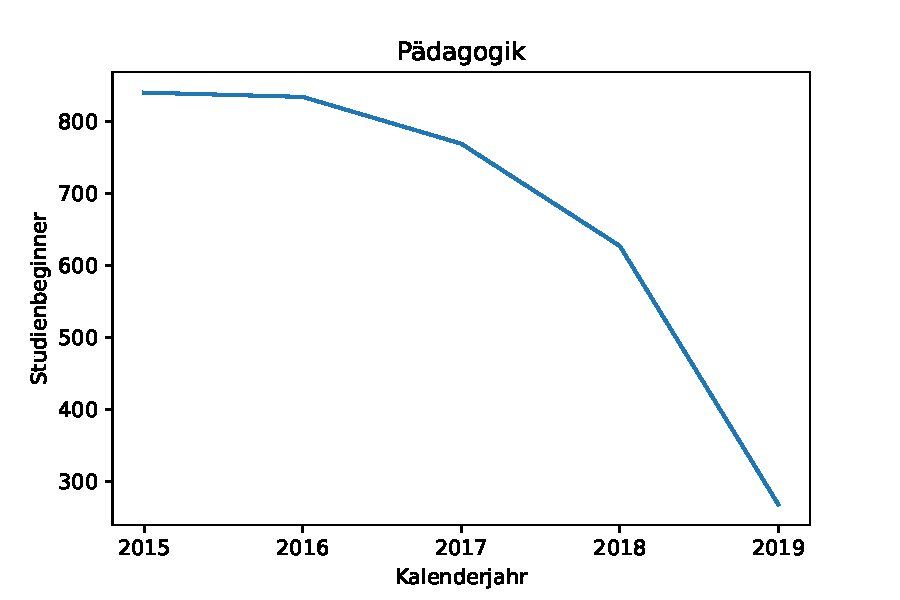
\includegraphics[width = 0.5\columnwidth]{pad3.pdf}
  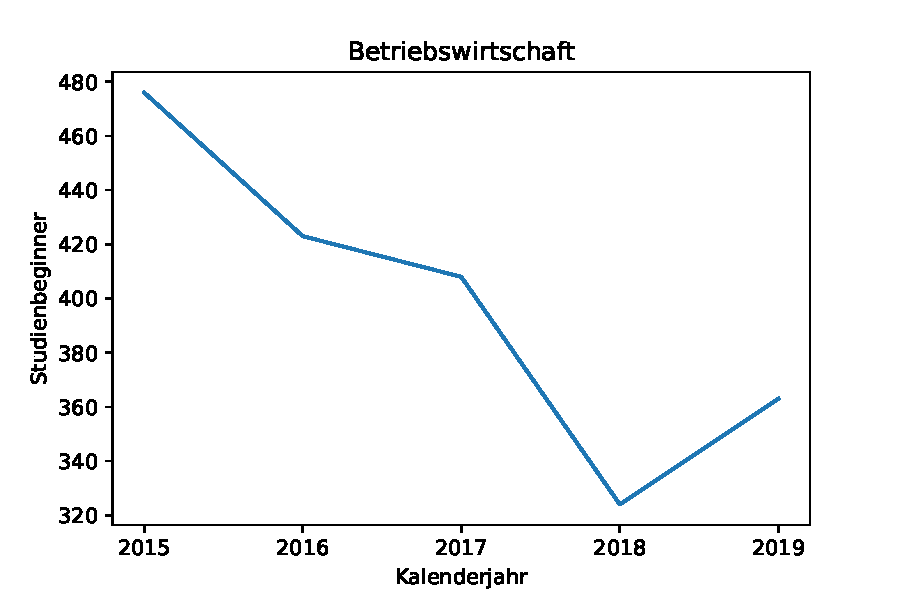
\includegraphics[width = 0.5\columnwidth]{bwl3.pdf}
  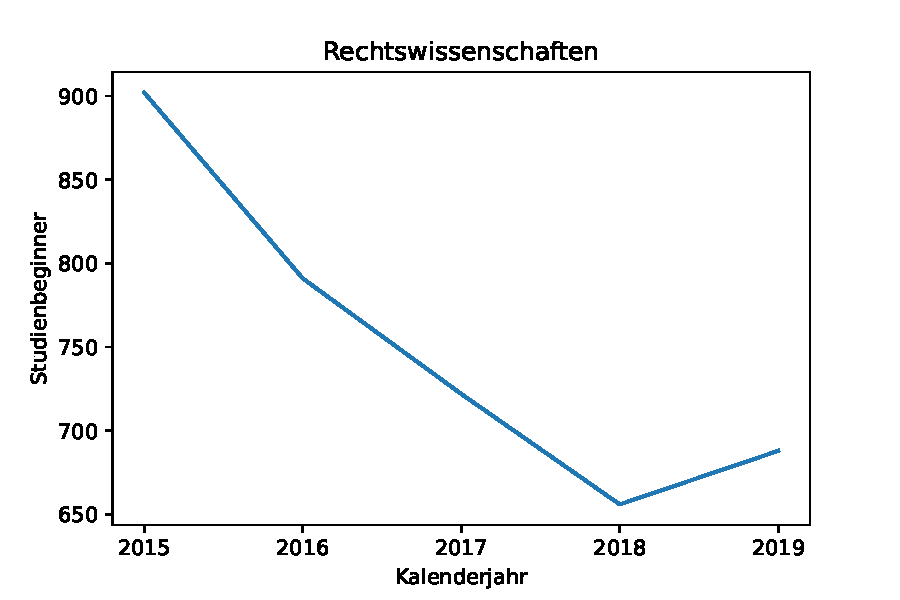
\includegraphics[width = 0.5\columnwidth]{jus3.pdf}
  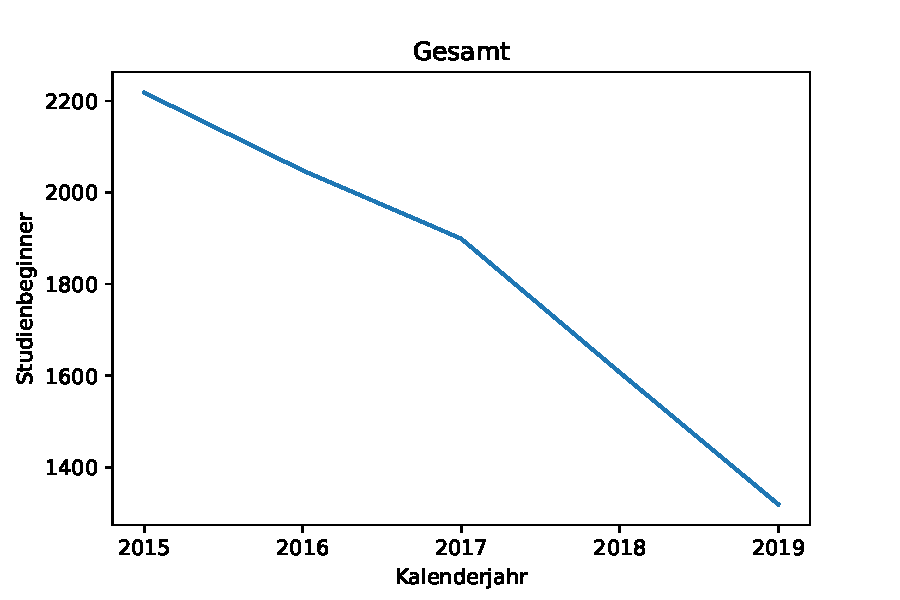
\includegraphics[width = 0.5\columnwidth]{ges3.pdf}
  \caption[Anzahl der Studienbeginner nach Fach und Kalenderjahr]{Hier werden die Anzahlen an Studienbeginnern je nach Fach und Kalenderjahr dargestellt.}
\end{figure}

Um einen besseren Einblick in die Zahlen der Studierenden nach Studienjahr und Kalenderjahr zu bekommen, sind in \hyperref[tab:numbers]{Tabelle 1.2} s\"amtliche
Zahlen nach Studienrichtung angef\"uhrt.

\begin{table}[ht]
  \caption{\label{tab:numbers} Anzahl der Studierenden nach Studienrichtung, Kalenderjahr und Studienjahr}
  \begin{tabular}{ p{1.5cm} p{1cm} p{1cm} p{1cm} p{1cm} p{1cm} p{1cm} p{1cm} p{1cm} p {1.5cm} }
    \toprule
                    &     & Jahr 1 & Jahr 2 & Jahr 3 & Jahr 4 & Jahr 5 & Jahr 6 & Jahr > 7 & \textbf{Gesamt} \\
    \midrule
    \multirow{3}{3em}{2015$/$16}
                    & JUS & 902    & 667    & 475    & 409    & 397    & 382    & 1253     & 4485            \\
                    & BWL & 476    & 353    & 231    & 355    & 153    & 104    & 399      & 2071            \\
                    & PAD & 804    & 567    & 415    & 270    & 115    & 48     & 115      & 2370            \\
    \midrule
    \multirow{3}{3em}{2016$/$17}
                    & JUS & 791    & 668    & 479    & 404    & 363    & 333    & 1285     & 4323            \\
                    & BWL & 423    & 357    & 308    & 177    & 181    & 73     & 374      & 1893            \\
                    & PAD & 834    & 538    & 419    & 282    & 122    & 57     & 126      & 2378            \\
    \midrule
    \multirow{3}{3em}{2017$/$18}
                    & JUS & 722    & 579    & 501    & 401    & 368    & 291    & 1257     & 4119            \\
                    & BWL & 408    & 314    & 286    & 228    & 75     & 83     & 324      & 1718            \\
                    & PAD & 769    & 578    & 419    & 279    & 124    & 68     & 139      & 2376            \\
    \midrule
    \multirow{3}{3em}{2018$/$19}
                    & JUS & 656    & 541    & 413    & 413    & 360    & 294    & 1153     & 3830            \\
                    & BWL & 324    & 292    & 254    & 202    & 113    & 49     & 270      & 1504            \\
                    & PAD & 627    & 453    & 444    & 268    & 120    & 56     & 128      & 2106            \\
    \midrule
    \multirow{3}{3em}{2019$/$20}
                    & JUS & 688    & 502    & 386    & 363    & 367    & 296    & 1113     & 3715            \\
                    & BWL & 363    & 242    & 244    & 192    & 96     & 66     & 231      & 1434            \\
                    & PAD & 268    & 415    & 335    & 292    & 122    & 50     & 138      & 1620            \\
    \midrule
    \multirow{3}{3em}{Gesamt Jahre}
                    & JUS & 3759   & 2957   & 2254   & 1990   & 1855   & 1596   & 6061     & 20472           \\
                    & BWL & 1994   & 1558   & 1323   & 1154   & 618    & 375    & 1598     & 8620            \\
                    & PAD & 3302   & 2551   & 2032   & 1391   & 603    & 279    & 656      & 10850           \\
    \midrule
    \textbf{Gesamt} &     & 9091   & 7066   & 5609   & 4535   & 3076   & 2250   & 8315     & 39942           \\

    \bottomrule
  \end{tabular}

\end{table}




\begin{figure}[ht]
  \label{fig:abb4}
  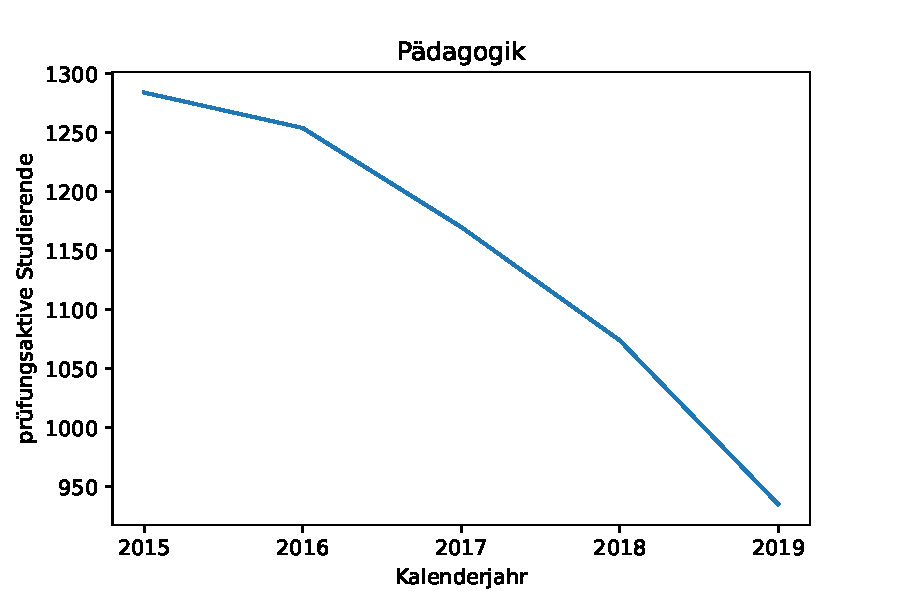
\includegraphics[width = 0.5\columnwidth]{pad4.pdf}
  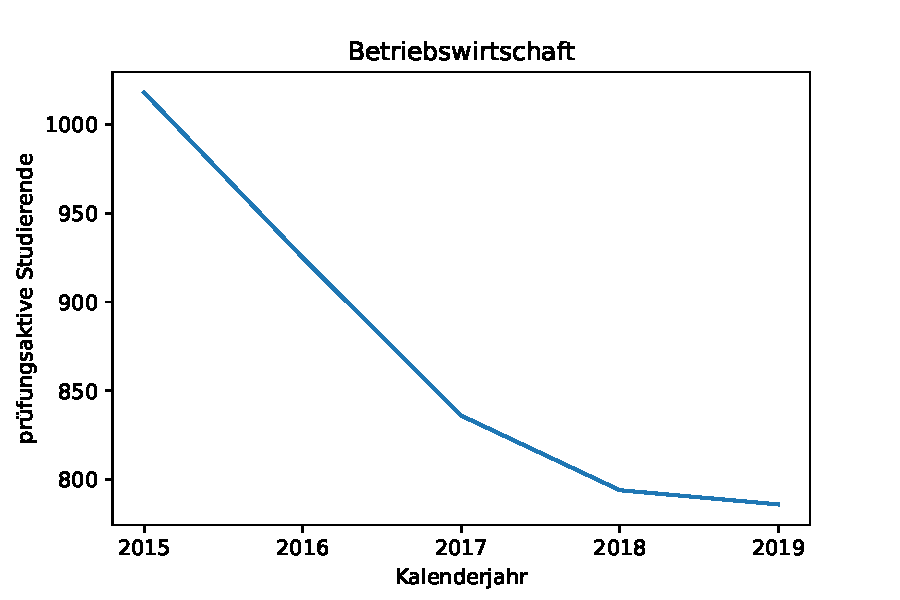
\includegraphics[width = 0.5\columnwidth]{bwl4.pdf}
  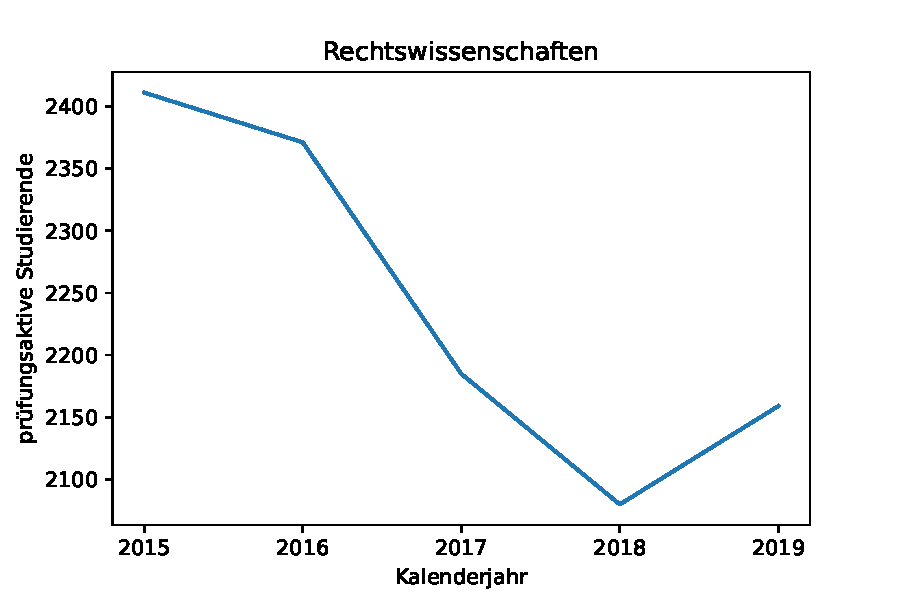
\includegraphics[width = 0.5\columnwidth]{jus4.pdf}
  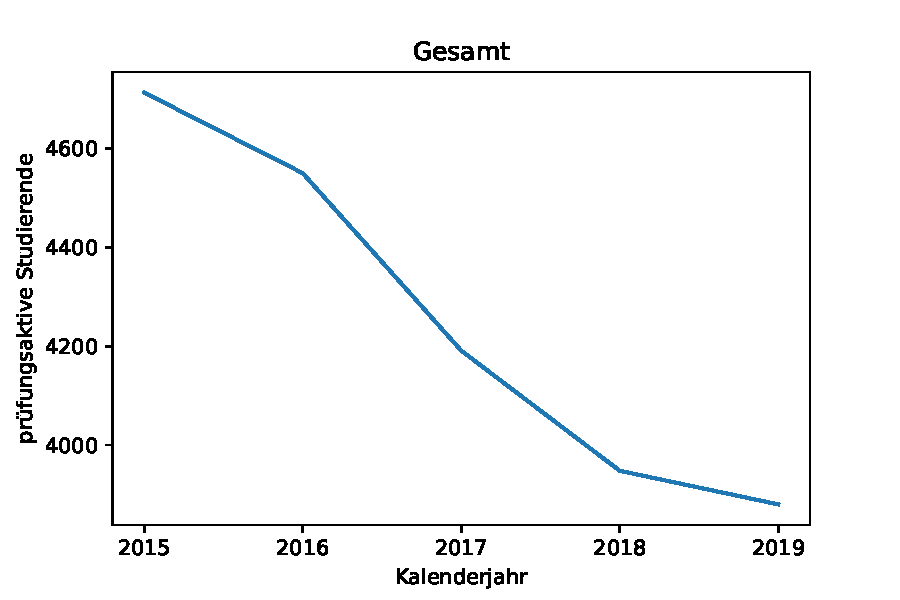
\includegraphics[width = 0.5\columnwidth]{ges4.pdf}
  \caption[prüfungsaktive Studierende nach Kalenderjahr]{Hier wird die Anzahl aller prüfungsaktiven Studierenden nach Kalenderjahr dargestellt. Das
    ist jene Zahl, die anschließend in der Zukunft geschätzt werden soll.}
\end{figure}


% \begin{figure}[ht]
%   \label{fig:abb5}
%   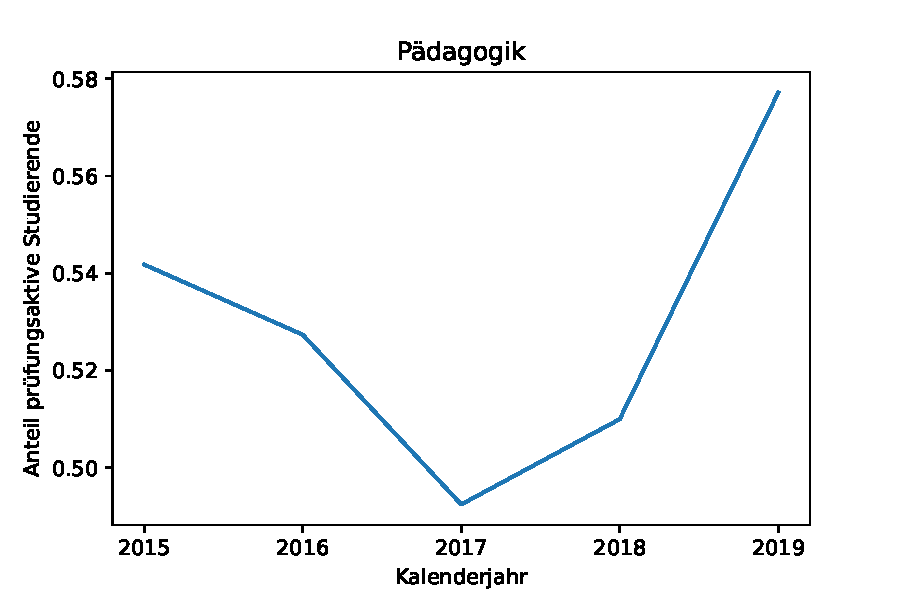
\includegraphics[width = 0.5\columnwidth]{pad5.pdf}
%   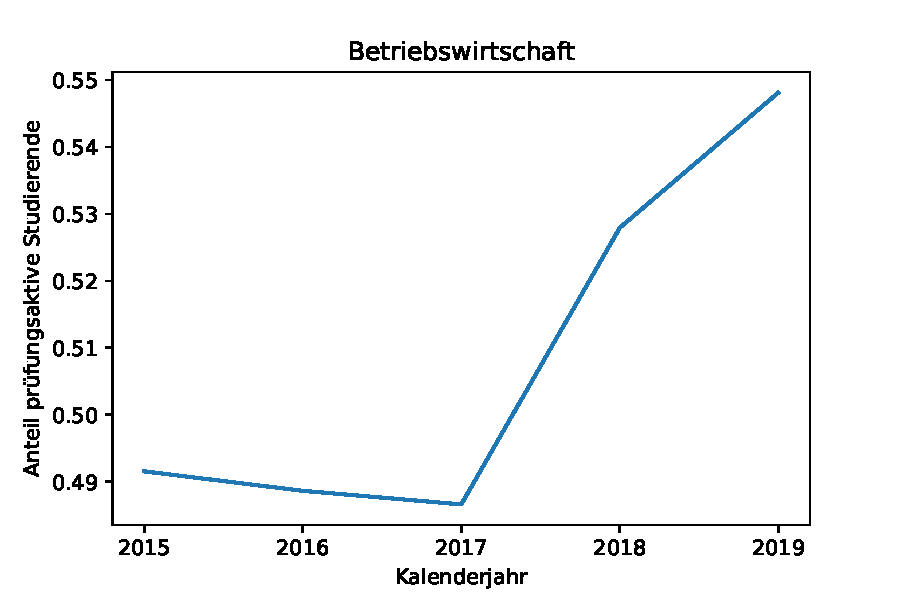
\includegraphics[width = 0.5\columnwidth]{bwl5.pdf}
%   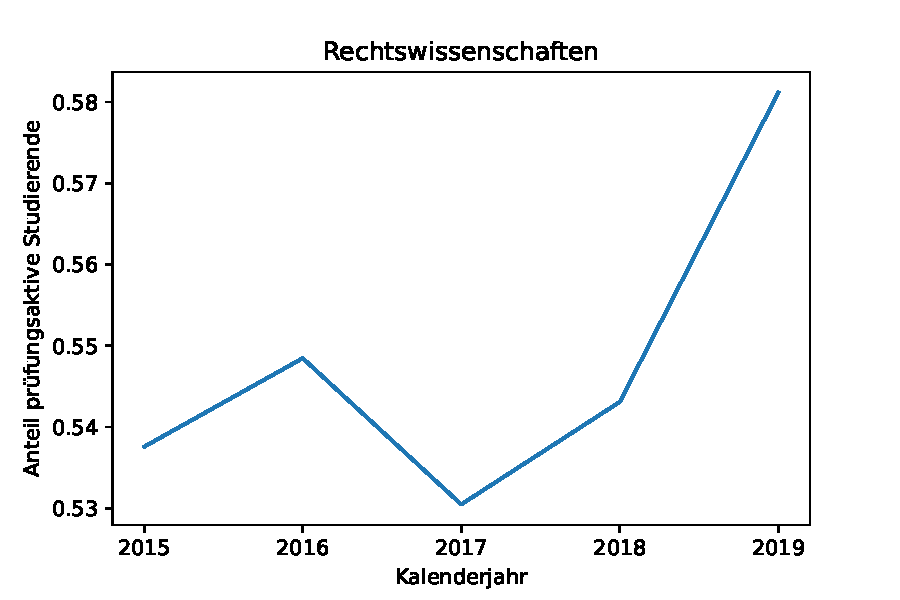
\includegraphics[width = 0.5\columnwidth]{jus5.pdf}
%   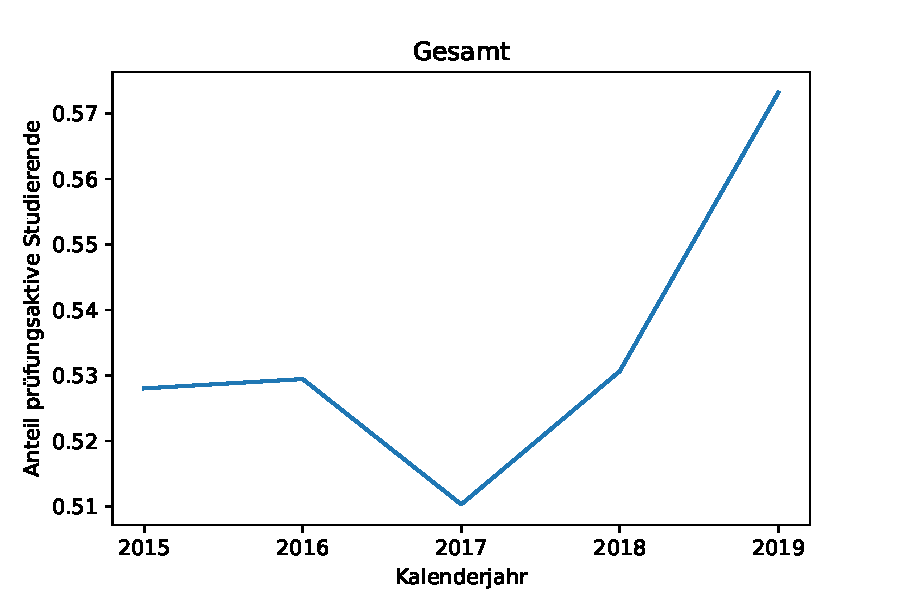
\includegraphics[width = 0.5\columnwidth]{ges5.pdf}
%   \caption[Anteil der prüfungsaktiven Studierenden nach Kalenderjahr]{Hier wird der Anteil an prüfungsaktiven Studierenden nach Kalenderjahr dargestellt.}
% \end{figure}









